\documentclass[aspectratio=169]{beamer}

\usetheme{default}
\usecolortheme{dove}

\setbeamertemplate{navigation symbols}{}
\setbeamertemplate{footline}{%
  \hfill{\large\insertframenumber\,/\,\inserttotalframenumber}\hspace{0.8em}\vspace{0.5em}%
}

\definecolor{popblue}{RGB}{52, 101, 164}
\definecolor{sampred}{RGB}{204, 0, 0}
\definecolor{paramgreen}{RGB}{0, 140, 70}
\definecolor{warnred}{RGB}{180, 40, 40}
\definecolor{orange1}{RGB}{220, 120, 0}
\definecolor{violet1}{RGB}{120, 50, 160}
\definecolor{lightbg}{RGB}{245, 245, 250}

\setbeamercolor{frametitle}{fg=popblue}
\setbeamercolor{title}{fg=popblue}

\usepackage{pgfplots}
\usepackage{tikz}
\usetikzlibrary{shapes, arrows.meta, positioning, calc, decorations.pathreplacing, patterns}
\pgfplotsset{compat=1.18}
\usepackage{amsmath, amssymb}
\usepackage{fontenc}

\title{Information Theory III: Advanced Topics for ML}
\subtitle{Data Processing Inequality $\cdot$ $f$-Divergences $\cdot$ ELBO $\cdot$ Information Bottleneck}
\date{}

\begin{document}

% ============================================================
\begin{frame}
\titlepage
\end{frame}

% ============================================================
\begin{frame}
\frametitle{Recap: What We Have So Far}

\begin{center}
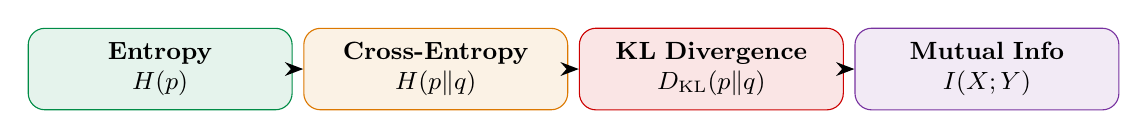
\begin{tikzpicture}[
  box/.style={draw=#1, fill=#1!10, rounded corners=6pt, minimum height=0.9cm, text width=3cm, align=center, font=\small, inner sep=5pt},
]
  \node[box=paramgreen] (ent) at (-5.2, 0.5) {\textbf{Entropy}\\$H(p)$};
  \node[box=orange1] (ce)  at (-1.7, 0.5) {\textbf{Cross-Entropy}\\$H(p\|q)$};
  \node[box=sampred] (kl)  at (1.8, 0.5) {\textbf{KL Divergence}\\$D_{\text{KL}}(p\|q)$};
  \node[box=violet1] (mi)  at (5.3, 0.5) {\textbf{Mutual Info}\\$I(X;Y)$};
  \draw[-{Stealth}, thick] (ent) -- (ce);
  \draw[-{Stealth}, thick] (ce) -- (kl);
  \draw[-{Stealth}, thick] (kl) -- (mi);
\end{tikzpicture}
\end{center}

\vspace{0.1cm}
\small
We established: cross-entropy loss = MLE, forward KL for supervised learning,
reverse KL for variational inference, MI for feature selection.

\vspace{0.2cm}
\begin{center}
\fcolorbox{popblue}{popblue!5}{\parbox{11cm}{\centering\small
  \textbf{Today:} Four powerful extensions.\\[3pt]
  \textbf{1.}~Data Processing Inequality \quad
  \textbf{2.}~$f$-Divergences \& GANs\\[2pt]
  \textbf{3.}~ELBO \& VAEs \quad
  \textbf{4.}~Information Bottleneck
}}
\end{center}
\end{frame}

% ============================================================
\section{Data Processing Inequality}

\begin{frame}
\begin{center}
\vspace{1cm}
{\LARGE\bfseries\textcolor{popblue}{Data Processing Inequality}}\\[15pt]
{\large Processing data can only \textbf{destroy} information, never create it.}
\end{center}
\end{frame}

% ============================================================
\begin{frame}
\frametitle{Markov Chains and Information Flow}

\small
A \textbf{Markov chain} $X \to Y \to Z$ means: $Z$ depends on $X$ only through $Y$.

$$p(x, y, z) = p(x)\,p(y \mid x)\,p(z \mid y)$$

\vspace{0.1cm}
\begin{center}
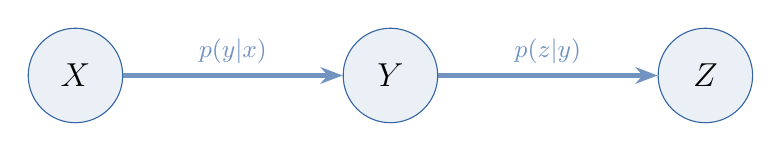
\begin{tikzpicture}[
  nd/.style={draw=popblue, fill=popblue!10, circle, minimum size=1.2cm, font=\large\bfseries, inner sep=0pt},
  arr/.style={-{Stealth[length=8pt]}, line width=2pt, popblue!70},
]
  \node[nd] (x) at (0, 0) {$X$};
  \node[nd] (y) at (4, 0) {$Y$};
  \node[nd] (z) at (8, 0) {$Z$};
  \draw[arr] (x) -- (y) node[midway, above, font=\small] {$p(y|x)$};
  \draw[arr] (y) -- (z) node[midway, above, font=\small] {$p(z|y)$};
\end{tikzpicture}
\end{center}

\vspace{0.2cm}
\textbf{Examples in ML:}
\begin{itemize}\setlength{\itemsep}{3pt}
  \item Raw pixels $\to$ convolutional features $\to$ class prediction
  \item Original data $\to$ PCA projection $\to$ clustering
  \item Text $\to$ embedding $\to$ classifier output
\end{itemize}
\end{frame}

% ============================================================
\begin{frame}
\frametitle{The Data Processing Inequality (DPI)}

\begin{center}
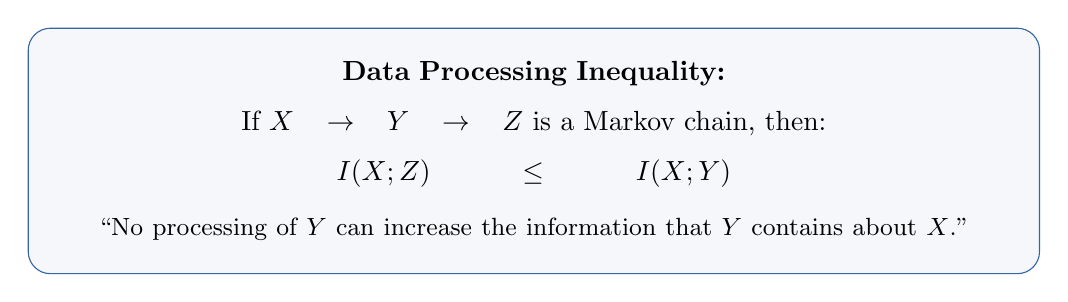
\begin{tikzpicture}
  \node[draw=popblue, fill=popblue!5, rounded corners=8pt, text width=12cm, align=center, inner sep=12pt] {
    \textbf{Data Processing Inequality:}\\[6pt]
    If $X \to Y \to Z$ is a Markov chain, then:\\[6pt]
    $I(X; Z) \;\leq\; I(X; Y)$\\[8pt]
    \small ``No processing of $Y$ can increase the information that $Y$ contains about $X$.''
  };
\end{tikzpicture}
\end{center}

\pause
\vspace{0.1cm}
\textbf{Proof sketch:}\\[2pt]
\small
Chain rule: $I(X;\, Y, Z) = I(X; Y) + I(X; Z \mid Y) = I(X; Z) + I(X; Y \mid Z)$.\\[2pt]
Since $X \to Y \to Z$: $\;I(X; Z \mid Y) = 0$, so $I(X; Y) = I(X; Z) + \underbrace{I(X; Y \mid Z)}_{\geq\, 0} \geq I(X; Z)$. \;$\square$

\vspace{0.05cm}
\begin{center}
\small Equality iff $Z$ is a \textbf{sufficient statistic} for $X$ w.r.t.\ $Y$.
\end{center}
\end{frame}

% ============================================================
\begin{frame}
\frametitle{DPI in Neural Networks}

\small
A feedforward network with layers $\mathbf{h}_1, \mathbf{h}_2, \ldots, \mathbf{h}_L$:

\vspace{0.1cm}
\begin{center}
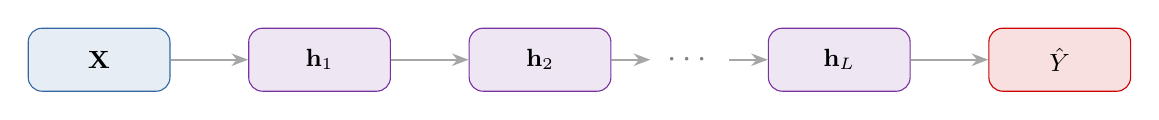
\begin{tikzpicture}[
  nd/.style={draw=#1, fill=#1!12, rounded corners=5pt, minimum width=1.8cm, minimum height=0.8cm, align=center, font=\small\bfseries},
  arr/.style={-{Stealth[length=6pt]}, thick, gray!70},
]
  \node[nd=popblue] (x) at (0, 0) {$\mathbf{X}$};
  \node[nd=violet1] (h1) at (2.8, 0) {$\mathbf{h}_1$};
  \node[nd=violet1] (h2) at (5.6, 0) {$\mathbf{h}_2$};
  \node[font=\large, gray] at (7.5, 0) {$\cdots$};
  \node[nd=violet1] (hl) at (9.4, 0) {$\mathbf{h}_L$};
  \node[nd=sampred] (y) at (12.2, 0) {$\hat{Y}$};
  \draw[arr] (x) -- (h1);
  \draw[arr] (h1) -- (h2);
  \draw[arr] (h2) -- (7, 0);
  \draw[arr] (8, 0) -- (hl);
  \draw[arr] (hl) -- (y);
\end{tikzpicture}
\end{center}

\vspace{0.1cm}
Each layer forms a Markov chain: $\;\mathbf{X} \to \mathbf{h}_1 \to \mathbf{h}_2 \to \cdots \to \mathbf{h}_L \to \hat{Y}$.

\vspace{0.1cm}
By DPI applied repeatedly:

\vspace{-0.2cm}
$$I(\mathbf{X};\, \mathbf{h}_1) \;\geq\; I(\mathbf{X};\, \mathbf{h}_2) \;\geq\; \cdots \;\geq\; I(\mathbf{X};\, \mathbf{h}_L) \;\geq\; I(\mathbf{X};\, \hat{Y})$$

\vspace{0.1cm}
\begin{center}
\fcolorbox{sampred}{sampred!5}{\parbox{11cm}{\centering\small
  \textbf{Each layer can only lose information about the input.}\\[3pt]
  The network must learn to keep what matters (about $Y$) and discard what doesn't.\\[2pt]
  This is exactly the \textbf{information bottleneck} idea (coming later).
}}
\end{center}
\end{frame}

% ============================================================
\begin{frame}
\frametitle{DPI: Practical Consequences}

\small
\begin{center}
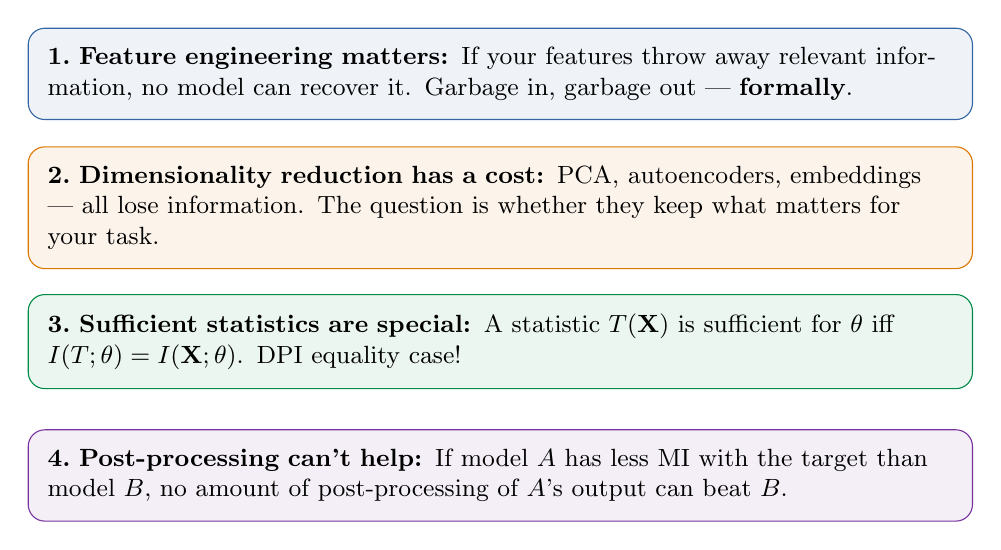
\begin{tikzpicture}[
  box/.style={draw=#1, fill=#1!8, rounded corners=6pt, text width=11.5cm, align=left, inner sep=7pt, font=\small},
]
  \node[box=popblue] at (0, 2.2) {
    \textbf{1.~Feature engineering matters:} If your features throw away relevant
    information, no model can recover it. Garbage in, garbage out --- \textbf{formally}.
  };
  \node[box=orange1] at (0, 0.5) {
    \textbf{2.~Dimensionality reduction has a cost:} PCA, autoencoders, embeddings ---
    all lose information. The question is whether they keep what matters for your task.
  };
  \node[box=paramgreen] at (0, -1.2) {
    \textbf{3.~Sufficient statistics are special:} A statistic $T(\mathbf{X})$ is sufficient
    for $\theta$ iff $I(T; \theta) = I(\mathbf{X}; \theta)$. DPI equality case!
  };
  \node[box=violet1] at (0, -2.9) {
    \textbf{4.~Post-processing can't help:} If model $A$ has less MI with the target
    than model $B$, no amount of post-processing of $A$'s output can beat $B$.
  };
\end{tikzpicture}
\end{center}
\end{frame}

% ============================================================
\section{$f$-Divergences}

\begin{frame}
\begin{center}
\vspace{1cm}
{\LARGE\bfseries\textcolor{popblue}{$f$-Divergences}}\\[15pt]
{\large KL divergence is just one member of a large family.}\\[4pt]
{\large The right divergence depends on the task.}
\end{center}
\end{frame}

% ============================================================
\begin{frame}
\frametitle{The $f$-Divergence Family}

\small
\begin{center}
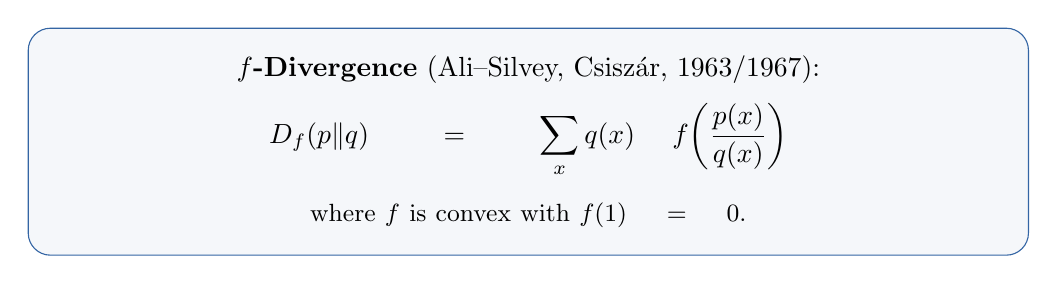
\begin{tikzpicture}
  \node[draw=popblue, fill=popblue!5, rounded corners=8pt, text width=12cm, align=center, inner sep=10pt] {
    \textbf{$f$-Divergence} (Ali--Silvey, Csisz\'{a}r, 1963/1967):\\[6pt]
    $D_f(p \| q) \;=\; \displaystyle\sum_{x} q(x)\; f\!\left(\frac{p(x)}{q(x)}\right)$\\[8pt]
    \small where $f$ is convex with $f(1) = 0$.
  };
\end{tikzpicture}
\end{center}

\vspace{0.2cm}
\textbf{Key properties} (inherited from convexity of $f$):
\begin{itemize}\setlength{\itemsep}{3pt}
  \item $D_f(p \| q) \geq 0$ always, with equality iff $p = q$
  \item \textbf{Satisfies DPI:} If $X \to Y$, then $D_f(p_Y \| q_Y) \leq D_f(p_X \| q_X)$
  \item Joint convexity in $(p, q)$
\end{itemize}

\vspace{0.1cm}
\begin{center}
\fcolorbox{orange1}{orange1!5}{\parbox{11cm}{\centering\small
  Different choices of $f$ give different divergences --- each with different
  sensitivities to where $p$ and $q$ disagree.
}}
\end{center}
\end{frame}

% ============================================================
\begin{frame}
\frametitle{The Family Members}

\small
\vspace{-0.1cm}
\begin{center}
\footnotesize
\renewcommand{\arraystretch}{1.5}
\begin{tabular}{llll}
  \textbf{Name} & \textbf{$f(t)$} & \textbf{Formula} & \textbf{ML use} \\
  \hline
  KL & $t\log t$ & $\sum p\log\frac{p}{q}$ & MLE, VI \\
  Reverse KL & $-\log t$ & $\sum q\log\frac{q}{p}$ & Variational inference \\
  Total Variation & $\frac{1}{2}|t - 1|$ & $\frac{1}{2}\sum|p - q|$ & Robustness \\
  Chi-squared & $(t-1)^2$ & $\sum\frac{(p-q)^2}{q}$ & Goodness-of-fit \\
  \textbf{Jensen--Shannon} & (see below) & $\frac{1}{2}D_{\text{KL}}(p\|m) + \frac{1}{2}D_{\text{KL}}(q\|m)$ & \textbf{GANs} \\
  Hellinger & $(\sqrt{t} - 1)^2$ & $\sum(\sqrt{p} - \sqrt{q})^2$ & Density estimation \\
  \hline
\end{tabular}
\end{center}

\vspace{0.1cm}
\begin{center}
\small JS: $f(t) = -\frac{t+1}{2}\log\frac{t+1}{2} + \frac{t\log t}{2}$, \quad $m = \frac{p+q}{2}$.
\end{center}
\end{frame}

% ============================================================
\begin{frame}
\frametitle{Jensen--Shannon Divergence: The Symmetric KL}

\small
KL divergence has two problems: it's \textbf{asymmetric} and \textbf{unbounded}.
Jensen--Shannon fixes both:

\vspace{0.1cm}
\begin{center}

\begin{tikzpicture}
  \node[draw=popblue, fill=popblue!5, rounded corners=8pt, text width=12cm, align=center, inner sep=10pt] {
    $\text{JSD}(p \| q) \;=\; \frac{1}{2}\,D_{\text{KL}}\!\left(p \;\middle\|\; \frac{p+q}{2}\right) + \frac{1}{2}\,D_{\text{KL}}\!\left(q \;\middle\|\; \frac{p+q}{2}\right)$
  };
\end{tikzpicture}
\end{center}

\vspace{0.15cm}
\begin{columns}[T]
\begin{column}{0.48\textwidth}
\textbf{Properties:}
\begin{itemize}\setlength{\itemsep}{3pt}
  \item \textcolor{paramgreen}{\checkmark} Symmetric: $\text{JSD}(p\|q) = \text{JSD}(q\|p)$
  \item \textcolor{paramgreen}{\checkmark} Bounded: $0 \leq \text{JSD} \leq \log 2$
  \item \textcolor{paramgreen}{\checkmark} $\sqrt{\text{JSD}}$ is a true metric
  \item \textcolor{paramgreen}{\checkmark} Always finite (even when supports differ)
\end{itemize}
\end{column}
\begin{column}{0.48\textwidth}
\vspace{0.1cm}
\textbf{Compare to KL:}
\begin{itemize}\setlength{\itemsep}{3pt}
  \item \textcolor{sampred}{\textbf{$\times$}} KL: asymmetric
  \item \textcolor{sampred}{\textbf{$\times$}} KL: unbounded ($\to\infty$)
  \item \textcolor{sampred}{\textbf{$\times$}} KL: $\infty$ when $q(x)=0, p(x)>0$
\end{itemize}
\end{column}
\end{columns}

\vspace{0.05cm}
\begin{center}
\fcolorbox{violet1}{violet1!5}{\parbox{11cm}{\centering\small
  \textbf{Intuition:} Instead of comparing $p$ to $q$ directly,
  both $p$ and $q$ are compared to their average $m = \frac{p+q}{2}$.
}}
\end{center}
\end{frame}

% ============================================================
\begin{frame}
\frametitle{$f$-Divergences and GANs}

\small
The original GAN (Goodfellow et al., 2014) trains a generator $G$ and discriminator $D$:

\vspace{-0.1cm}
$$\min_G \max_D \;\; \mathbb{E}_{x \sim p_{\text{data}}}[\log D(x)] + \mathbb{E}_{z \sim p_z}[\log(1 - D(G(z)))]$$

\pause
\vspace{0.05cm}
\textbf{Key result:} For optimal $D^*$, the GAN objective becomes:

\vspace{-0.2cm}
$$\min_G \;\; 2\,\text{JSD}(p_{\text{data}} \| p_G) - \log 4$$

\vspace{0.1cm}
\begin{center}
\fcolorbox{paramgreen}{paramgreen!5}{\parbox{11cm}{\centering\small
  \textbf{Training a GAN = minimizing JS divergence between real and generated data.}
}}
\end{center}

\pause
\vspace{0.15cm}
\textbf{$f$-GAN} (Nowozin et al., 2016) generalizes this:

\vspace{0.05cm}
\begin{center}
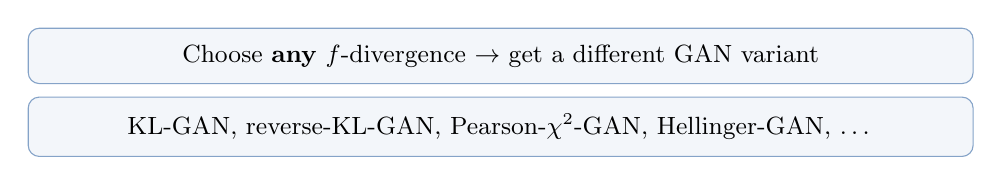
\begin{tikzpicture}[
  pbox/.style={draw=popblue!60, fill=popblue!6, rounded corners=4pt, minimum width=12cm, align=left, inner sep=6pt, font=\small}
]
  \node[pbox] at (0, 0.5) {Choose \textbf{any} $f$-divergence $\to$ get a different GAN variant};
  \node[pbox] at (0, -0.4) {KL-GAN, reverse-KL-GAN, Pearson-$\chi^2$-GAN, Hellinger-GAN, \ldots};
\end{tikzpicture}
\end{center}
\end{frame}

% ============================================================
\begin{frame}
\frametitle{When Divergences Differ: Support Mismatch}

\small
What happens when $p$ and $q$ have \textbf{different supports}?

\vspace{-0.05cm}
\begin{center}
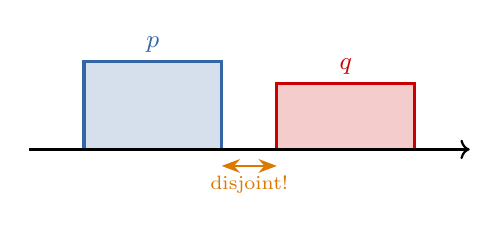
\begin{tikzpicture}[scale=0.7]
  \fill[popblue!20] (-3, 0) rectangle (-0.5, 1.6);
  \draw[very thick, popblue] (-3, 0) -- (-3, 1.6) -- (-0.5, 1.6) -- (-0.5, 0);
  \node[font=\small\bfseries, popblue] at (-1.75, 1.9) {$p$};
  \fill[sampred!20] (0.5, 0) rectangle (3, 1.2);
  \draw[very thick, sampred] (0.5, 0) -- (0.5, 1.2) -- (3, 1.2) -- (3, 0);
  \node[font=\small\bfseries, sampred] at (1.75, 1.5) {$q$};
  \draw[thick, ->] (-4, 0) -- (4, 0);
  \draw[{Stealth}-{Stealth}, thick, orange1] (-0.5, -0.3) -- (0.5, -0.3)
    node[midway, below, font=\scriptsize] {disjoint!};
\end{tikzpicture}
\end{center}

\vspace{-0.2cm}
\begin{center}
\renewcommand{\arraystretch}{1.2}
\small
\begin{tabular}{lcc}
  \textbf{Divergence} & \textbf{Disjoint value} & \textbf{Gradient?} \\
  \hline
  $D_{\text{KL}}(p \| q)$ & $+\infty$ & \textcolor{sampred}{\textbf{$\times$}} undefined \\
  Total Variation & $1$ (saturated) & \textcolor{sampred}{\textbf{$\times$}} zero \\
  $\text{JSD}(p \| q)$ & $\log 2$ (saturated) & \textcolor{sampred}{\textbf{$\times$}} zero \\
  \hline
\end{tabular}
\end{center}

\vspace{-0.05cm}
\begin{center}
\fcolorbox{warnred}{warnred!5}{\parbox{11cm}{\centering\small
  \textbf{This is why early GANs were hard to train!}
  JS gradients vanish when $p_{\text{data}}$ and $p_G$ have little overlap.
  Fix: \textbf{Wasserstein distance} --- always gives useful gradients.
}}
\end{center}
\end{frame}

% ============================================================
\section{ELBO and Variational Autoencoders}

\begin{frame}
\begin{center}
\vspace{1cm}
{\LARGE\bfseries\textcolor{popblue}{ELBO \& Variational Autoencoders}}\\[15pt]
{\large The reverse KL from Lecture 2 leads to}\\[4pt]
{\large the most important equation in generative modeling.}
\end{center}
\end{frame}

% ============================================================
\begin{frame}
\frametitle{The Problem: Intractable Posteriors}

\small
In a latent variable model, we want $p_\theta(\mathbf{x})$ --- the marginal likelihood:

\vspace{-0.2cm}
$$p_\theta(\mathbf{x}) = \int p_\theta(\mathbf{x} \mid \mathbf{z})\, p(\mathbf{z})\, d\mathbf{z}$$

\vspace{-0.1cm}
\begin{center}
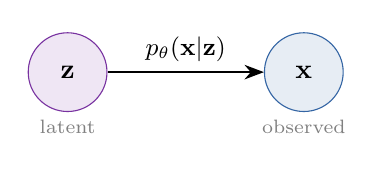
\begin{tikzpicture}[
  nd/.style={draw=#1, fill=#1!12, circle, minimum size=1cm, font=\normalsize\bfseries, inner sep=0pt},
  arr/.style={-{Stealth[length=7pt]}, thick},
]
  \node[nd=violet1] (z) at (0, 0) {$\mathbf{z}$};
  \node[nd=popblue] (x) at (3, 0) {$\mathbf{x}$};
  \draw[arr] (z) -- (x) node[midway, above, font=\small] {$p_\theta(\mathbf{x}|\mathbf{z})$};
  \node[font=\scriptsize, gray] at (0, -0.7) {latent};
  \node[font=\scriptsize, gray] at (3, -0.7) {observed};
\end{tikzpicture}
\end{center}

\vspace{0.05cm}
\textbf{Two problems:}
\begin{enumerate}\setlength{\itemsep}{1pt}
  \item The integral over $\mathbf{z}$ is usually \textbf{intractable} (no closed form).
  \item The posterior $p_\theta(\mathbf{z} \mid \mathbf{x}) = \frac{p_\theta(\mathbf{x}|\mathbf{z})\,p(\mathbf{z})}{p_\theta(\mathbf{x})}$ requires $p_\theta(\mathbf{x})$ --- circular!
\end{enumerate}

\vspace{0.1cm}
\begin{center}
\fcolorbox{orange1}{orange1!5}{\parbox{11cm}{\centering\small
  \textbf{Idea:} Approximate the intractable posterior $p_\theta(\mathbf{z}|\mathbf{x})$
  with a simple distribution $q_\phi(\mathbf{z}|\mathbf{x})$ --- using \textbf{reverse KL}.
}}
\end{center}
\end{frame}

% ============================================================
\begin{frame}
\frametitle{Deriving the ELBO}

\small
Start with the log-marginal likelihood and use any distribution $q_\phi(\mathbf{z}|\mathbf{x})$:

\vspace{-0.2cm}
\begin{align*}
  \log p_\theta(\mathbf{x}) &= \log \int p_\theta(\mathbf{x}, \mathbf{z})\, d\mathbf{z}
  = \log \int q_\phi(\mathbf{z}|\mathbf{x})\,\frac{p_\theta(\mathbf{x}, \mathbf{z})}{q_\phi(\mathbf{z}|\mathbf{x})}\, d\mathbf{z}\\[4pt]
  &\geq \int q_\phi(\mathbf{z}|\mathbf{x})\,\log\frac{p_\theta(\mathbf{x}, \mathbf{z})}{q_\phi(\mathbf{z}|\mathbf{x})}\, d\mathbf{z}
  \qquad\text{(Jensen's inequality)}
\end{align*}

\pause
\vspace{-0.2cm}
\begin{center}
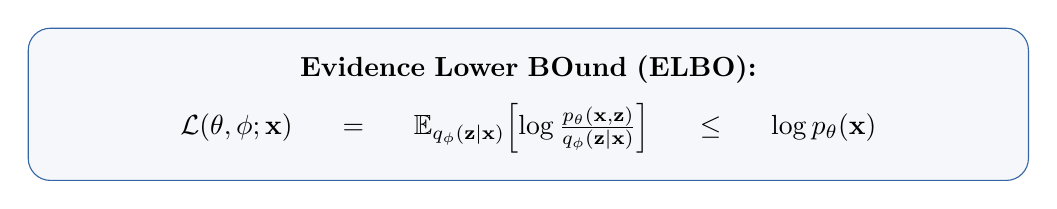
\begin{tikzpicture}
  \node[draw=popblue, fill=popblue!5, rounded corners=8pt, text width=12cm, align=center, inner sep=10pt] {
    \textbf{Evidence Lower BOund (ELBO):}\\[6pt]
    $\mathcal{L}(\theta, \phi; \mathbf{x}) \;=\; \mathbb{E}_{q_\phi(\mathbf{z}|\mathbf{x})}\!\left[\log\frac{p_\theta(\mathbf{x}, \mathbf{z})}{q_\phi(\mathbf{z}|\mathbf{x})}\right] \;\leq\; \log p_\theta(\mathbf{x})$
  };
\end{tikzpicture}
\end{center}

\vspace{0.15cm}
The \textbf{gap} between ELBO and log-evidence is exactly the reverse KL:

$$\boxed{\log p_\theta(\mathbf{x}) \;=\; \underbrace{\mathcal{L}(\theta, \phi; \mathbf{x})}_{\text{ELBO}} \;+\; \underbrace{D_{\text{KL}}\!\big(q_\phi(\mathbf{z}|\mathbf{x}) \;\|\; p_\theta(\mathbf{z}|\mathbf{x})\big)}_{\geq\; 0}}$$
\end{frame}

% ============================================================
\begin{frame}
\frametitle{ELBO = Reconstruction $-$ KL Penalty}

\small
Expanding the ELBO gives a beautiful decomposition:

\vspace{-0.1cm}
\begin{align*}
  \mathcal{L}(\theta, \phi; \mathbf{x})
  &= \mathbb{E}_{q_\phi(\mathbf{z}|\mathbf{x})}\!\left[\log p_\theta(\mathbf{x} | \mathbf{z})\right]
  - D_{\text{KL}}\!\big(q_\phi(\mathbf{z}|\mathbf{x}) \;\|\; p(\mathbf{z})\big)
\end{align*}

\vspace{0.1cm}
\begin{center}
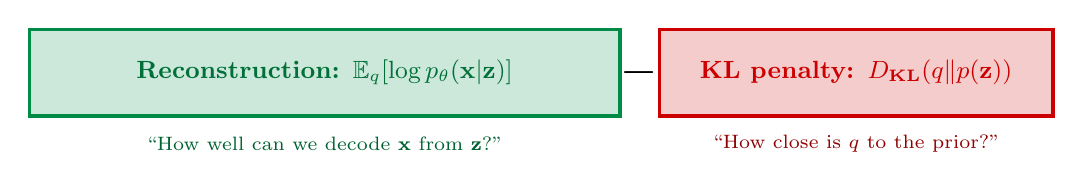
\begin{tikzpicture}
  % Full bar
  \fill[paramgreen!20] (0,0) rectangle (7.5, 1.1);
  \draw[very thick, paramgreen] (0,0) rectangle (7.5, 1.1);
  \node[font=\small\bfseries, paramgreen!80!black] at (3.75, 0.55) {Reconstruction: $\mathbb{E}_{q}[\log p_\theta(\mathbf{x}|\mathbf{z})]$};

  \fill[sampred!20] (8, 0) rectangle (13, 1.1);
  \draw[very thick, sampred] (8, 0) rectangle (13, 1.1);
  \node[font=\small\bfseries, sampred] at (10.5, 0.55) {KL penalty: $D_{\text{KL}}(q \| p(\mathbf{z}))$};

  % Labels below
  \node[font=\scriptsize, paramgreen!70!black] at (3.75, -0.35) {``How well can we decode $\mathbf{x}$ from $\mathbf{z}$?''};
  \node[font=\scriptsize, sampred!70!black] at (10.5, -0.35) {``How close is $q$ to the prior?''};

  % Minus sign
  \node[font=\LARGE\bfseries] at (7.75, 0.55) {$-$};
\end{tikzpicture}
\end{center}

\vspace{0.2cm}
\begin{center}
\fcolorbox{orange1}{orange1!5}{\parbox{11cm}{\centering\small
  \textbf{Maximize ELBO} = make reconstructions good (high $\log p_\theta(\mathbf{x}|\mathbf{z})$)
  while keeping $q_\phi(\mathbf{z}|\mathbf{x})$ close to the prior $p(\mathbf{z})$.\\[3pt]
  The KL penalty acts as a \textbf{regularizer} on the latent space.
}}
\end{center}
\end{frame}

% ============================================================
\begin{frame}
\frametitle{The Variational Autoencoder (VAE)}

\small
The VAE (Kingma \& Welling, 2014) implements the ELBO with neural networks:

\vspace{0.15cm}
\begin{center}
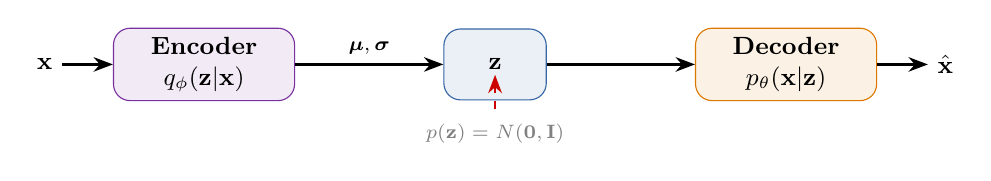
\begin{tikzpicture}[scale=0.88,
  block/.style={draw=#1, fill=#1!10, rounded corners=6pt, minimum width=2.3cm, minimum height=0.9cm, align=center, font=\small\bfseries},
  arr/.style={-{Stealth[length=7pt]}, thick},
]
  % Encoder
  \node[block=violet1] (enc) at (0, 0) {Encoder\\$q_\phi(\mathbf{z}|\mathbf{x})$};
  \node[block=popblue, minimum width=1.3cm] (z) at (4.2, 0) {$\mathbf{z}$};
  \node[block=orange1] (dec) at (8.4, 0) {Decoder\\$p_\theta(\mathbf{x}|\mathbf{z})$};

  % Input / output
  \node[font=\small] (x1) at (-2.3, 0) {$\mathbf{x}$};
  \node[font=\small] (x2) at (10.7, 0) {$\hat{\mathbf{x}}$};

  \draw[arr] (x1) -- (enc);
  \draw[arr] (enc) -- node[above, font=\scriptsize] {$\boldsymbol{\mu}, \boldsymbol{\sigma}$} (z);
  \draw[arr] (z) -- (dec);
  \draw[arr] (dec) -- (x2);

  % Prior arrow
  \node[font=\scriptsize, gray] at (4.2, -1) {$p(\mathbf{z}) = N(\mathbf{0}, \mathbf{I})$};
  \draw[thick, sampred, dashed, -{Stealth}] (4.2, -0.65) -- (4.2, -0.15);
\end{tikzpicture}
\end{center}

\vspace{0.2cm}
\begin{center}
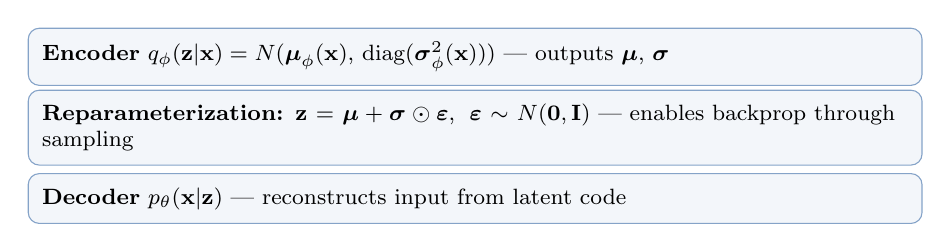
\begin{tikzpicture}[
  pbox/.style={draw=popblue!60, fill=popblue!6, rounded corners=4pt, text width=11cm, align=left, inner sep=5pt, font=\footnotesize}
]
  \node[pbox] at (0, 0.9) {\textbf{Encoder} $q_\phi(\mathbf{z}|\mathbf{x}) = N(\boldsymbol{\mu}_\phi(\mathbf{x}),\, \text{diag}(\boldsymbol{\sigma}_\phi^2(\mathbf{x})))$ --- outputs $\boldsymbol{\mu}$, $\boldsymbol{\sigma}$};
  \node[pbox] at (0, 0.0) {\textbf{Reparameterization:} $\mathbf{z} = \boldsymbol{\mu} + \boldsymbol{\sigma} \odot \boldsymbol{\varepsilon}$, \;$\boldsymbol{\varepsilon} \sim N(\mathbf{0}, \mathbf{I})$ --- enables backprop through sampling};
  \node[pbox] at (0, -0.9) {\textbf{Decoder} $p_\theta(\mathbf{x}|\mathbf{z})$ --- reconstructs input from latent code};
\end{tikzpicture}
\end{center}
\end{frame}

% ============================================================
\begin{frame}
\frametitle{VAE Loss = ELBO in Practice}

\small
For Gaussian encoder and prior, the KL term has a \textbf{closed form}:

$$D_{\text{KL}}\!\big(q_\phi(\mathbf{z}|\mathbf{x}) \| p(\mathbf{z})\big) = \frac{1}{2}\sum_{j=1}^d \left(\mu_j^2 + \sigma_j^2 - \log\sigma_j^2 - 1\right)$$

\vspace{0.1cm}
The reconstruction term depends on the output distribution:

\vspace{0.1cm}
\begin{center}
\renewcommand{\arraystretch}{1.5}
\begin{tabular}{lll}
  \textbf{Data type} & \textbf{$p_\theta(\mathbf{x}|\mathbf{z})$} & \textbf{Reconstruction loss} \\
  \hline
  Continuous & Gaussian & MSE: $\|\mathbf{x} - \hat{\mathbf{x}}\|^2$ \\
  Binary / images & Bernoulli & Binary cross-entropy \\
  \hline
\end{tabular}
\end{center}

\vspace{0.15cm}
\begin{center}
\fcolorbox{paramgreen}{paramgreen!5}{\parbox{11cm}{\centering\small
  \textbf{VAE loss} $= \underbrace{\text{Reconstruction error}}_{\text{MSE or BCE}}
  + \underbrace{\beta \cdot D_{\text{KL}}(q_\phi \| p)}_{\text{latent regularizer}}$\\[5pt]
  $\beta = 1$: standard VAE. \quad $\beta > 1$: $\beta$-VAE (disentangled representations).
}}
\end{center}
\end{frame}

% ============================================================
\begin{frame}
\frametitle{The ELBO Landscape}

\small
\begin{center}
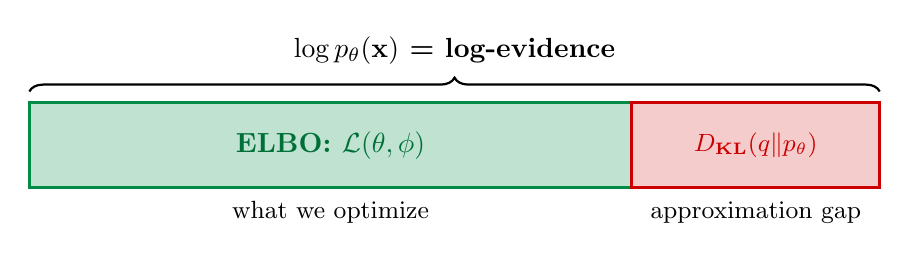
\begin{tikzpicture}[scale=0.9]
  % Evidence bar
  \fill[popblue!15] (0, 0) rectangle (12, 1.2);
  \draw[very thick, popblue] (0, 0) rectangle (12, 1.2);

  % ELBO portion
  \fill[paramgreen!25] (0, 0) rectangle (8.5, 1.2);
  \draw[very thick, paramgreen] (0, 0) rectangle (8.5, 1.2);
  \node[font=\normalsize\bfseries, paramgreen!80!black] at (4.25, 0.6) {ELBO: $\mathcal{L}(\theta, \phi)$};

  % KL gap
  \fill[sampred!20] (8.5, 0) rectangle (12, 1.2);
  \draw[very thick, sampred] (8.5, 0) rectangle (12, 1.2);
  \node[font=\small\bfseries, sampred] at (10.25, 0.6) {$D_{\text{KL}}(q\|p_\theta)$};

  % Labels
  \node[font=\small] at (4.25, -0.35) {what we optimize};
  \node[font=\small] at (10.25, -0.35) {approximation gap};

  % Top brace
  \draw[decorate, decoration={brace, amplitude=5pt, raise=4pt}, thick]
    (0, 1.2) -- (12, 1.2) node[midway, above, yshift=10pt, font=\normalsize\bfseries] {$\log p_\theta(\mathbf{x})$ = log-evidence};
\end{tikzpicture}
\end{center}

\vspace{0.2cm}
\begin{center}
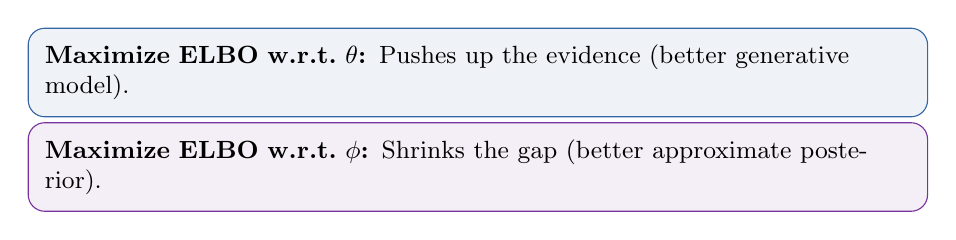
\begin{tikzpicture}[
  box/.style={draw=#1, fill=#1!8, rounded corners=6pt, text width=11cm, align=left, inner sep=6pt, font=\small},
]
  \node[box=popblue] at (0, 0.7) {
    \textbf{Maximize ELBO w.r.t.\ $\theta$:} Pushes up the evidence (better generative model).
  };
  \node[box=violet1] at (0, -0.5) {
    \textbf{Maximize ELBO w.r.t.\ $\phi$:} Shrinks the gap (better approximate posterior).
  };
\end{tikzpicture}
\end{center}
\end{frame}

% ============================================================
\section{Information Bottleneck}

\begin{frame}
\begin{center}
\vspace{1cm}
{\LARGE\bfseries\textcolor{popblue}{The Information Bottleneck}}\\[15pt]
{\large Compress the input. Preserve what matters for the task.}\\[4pt]
{\large A principled theory of representation learning.}
\end{center}
\end{frame}

% ============================================================
\begin{frame}
\frametitle{The Information Bottleneck Principle}

\small
Setup: input $X$, target $Y$, and a representation $T$ that compresses $X$.

\vspace{0.1cm}
\begin{center}
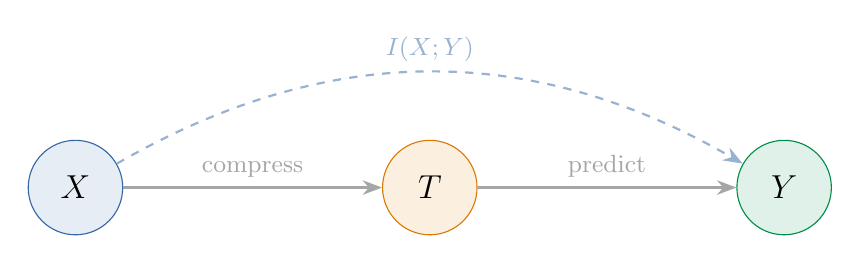
\begin{tikzpicture}[
  nd/.style={draw=#1, fill=#1!12, circle, minimum size=1.2cm, font=\large\bfseries, inner sep=0pt},
  arr/.style={-{Stealth[length=7pt]}, thick, gray!70},
]
  \node[nd=popblue] (x) at (0, 0) {$X$};
  \node[nd=orange1] (t) at (4.5, 0) {$T$};
  \node[nd=paramgreen] (y) at (9, 0) {$Y$};
  \draw[arr] (x) -- (t) node[midway, above, font=\small] {compress};
  \draw[arr] (t) -- (y) node[midway, above, font=\small] {predict};
  \draw[arr, dashed, popblue!50] (x) to[bend left=30] node[midway, above, font=\small] {$I(X;Y)$} (y);
\end{tikzpicture}
\end{center}

\vspace{0.1cm}
\begin{center}
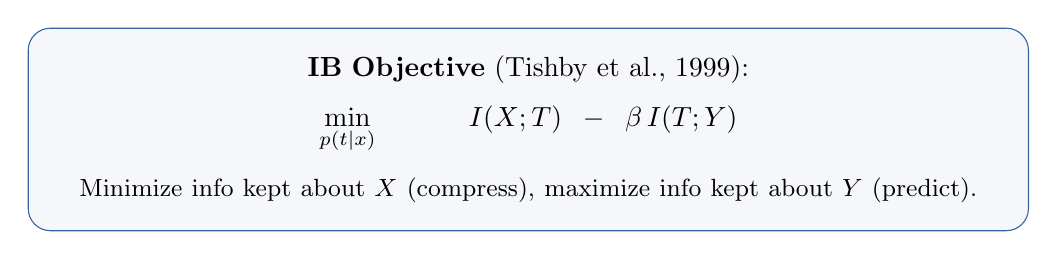
\begin{tikzpicture}
  \node[draw=popblue, fill=popblue!5, rounded corners=8pt, text width=12cm, align=center, inner sep=10pt] {
    \textbf{IB Objective} (Tishby et al., 1999):\\[6pt]
    $\displaystyle\min_{p(t|x)} \;\; I(X; T) - \beta\, I(T; Y)$\\[8pt]
    \small Minimize info kept about $X$ (compress), maximize info kept about $Y$ (predict).
  };
\end{tikzpicture}
\end{center}

\vspace{0.1cm}
\begin{center}
\small $\beta > 0$ is a Lagrange multiplier controlling the compression--prediction tradeoff.
\end{center}
\end{frame}

% ============================================================
\begin{frame}
\frametitle{The Information Plane}

\small
Each representation $T$ can be plotted as a point $\big(I(X;T),\; I(T;Y)\big)$:

\vspace{0.1cm}
\begin{center}
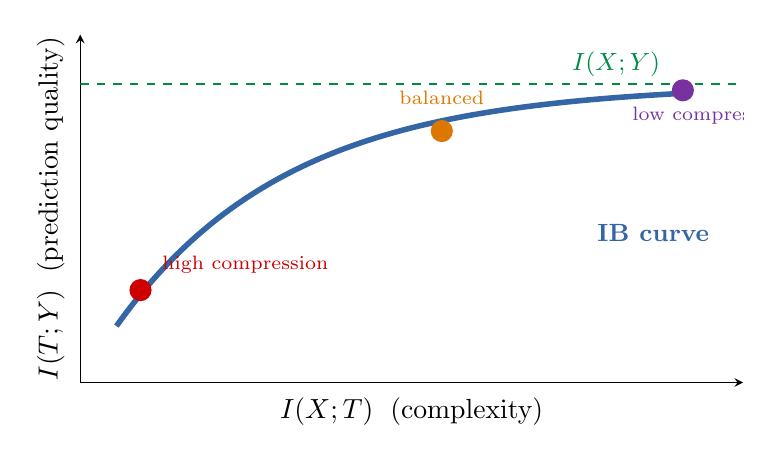
\begin{tikzpicture}
  \begin{axis}[
    width=10cm, height=6cm,
    xlabel={$I(X; T)$ \;(complexity)},
    ylabel={$I(T; Y)$ \;(prediction quality)},
    xmin=0, xmax=5.5,
    ymin=0, ymax=3.5,
    xtick=\empty, ytick=\empty,
    axis lines=left,
    every axis plot/.append style={line width=2pt},
  ]
    % IB curve
    \addplot[popblue, smooth, samples=100, domain=0.3:5] {3*(1 - exp(-0.7*x))};

    % I(X;Y) ceiling
    \draw[dashed, thick, paramgreen] (axis cs:0, 3) -- (axis cs:5.5, 3);
    \node[font=\small\bfseries, paramgreen, anchor=west] at (axis cs:4, 3.2) {$I(X;Y)$};

    % Points on curve
    \fill[sampred] (axis cs:0.5, 0.93) circle (4pt);
    \node[font=\scriptsize, sampred, anchor=south west] at (axis cs:0.6, 1.0) {high compression};

    \fill[orange1] (axis cs:3, 2.53) circle (4pt);
    \node[font=\scriptsize, orange1, anchor=south] at (axis cs:3, 2.7) {balanced};

    \fill[violet1] (axis cs:5, 2.94) circle (4pt);
    \node[font=\scriptsize, violet1, anchor=south west] at (axis cs:4.5, 2.5) {low compression};

    % Curve label
    \node[font=\small\bfseries, popblue, anchor=east] at (axis cs:5.3, 1.5) {IB curve};
  \end{axis}
\end{tikzpicture}
\end{center}

\vspace{-0.2cm}
\begin{center}
\small The IB curve traces optimal tradeoffs. Points below it are suboptimal.\\
$\beta$ moves you along the curve: small $\beta \to$ more compression, large $\beta \to$ more prediction.
\end{center}
\end{frame}

% ============================================================
\begin{frame}
\frametitle{IB and Deep Learning (Tishby \& Zaslavsky, 2015)}

\small
\textbf{Claim:} Deep networks implicitly optimize the IB tradeoff.

\vspace{0.1cm}
Each hidden layer $\mathbf{h}_\ell$ defines a point in the information plane:

\vspace{0.15cm}
\begin{center}
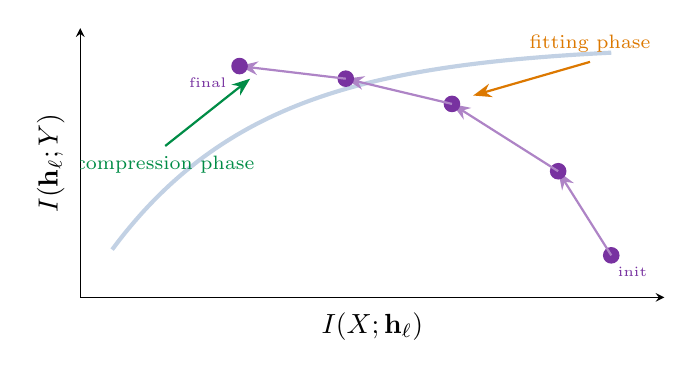
\begin{tikzpicture}
  \begin{axis}[
    width=9cm, height=5cm,
    xlabel={$I(X; \mathbf{h}_\ell)$},
    ylabel={$I(\mathbf{h}_\ell; Y)$},
    xmin=0, xmax=5.5,
    ymin=0, ymax=3.2,
    xtick=\empty, ytick=\empty,
    axis lines=left,
  ]
    % IB curve (faint)
    \addplot[popblue!30, smooth, samples=100, domain=0.3:5, line width=1.5pt] {3*(1 - exp(-0.7*x))};

    % Training trajectory (layers)
    \fill[violet1] (axis cs:5, 0.5) circle (3pt);
    \node[font=\tiny, violet1] at (axis cs:5.2, 0.3) {init};

    \draw[-{Stealth}, thick, violet1!60] (axis cs:5, 0.5) -- (axis cs:4.5, 1.5);
    \fill[violet1] (axis cs:4.5, 1.5) circle (3pt);

    \draw[-{Stealth}, thick, violet1!60] (axis cs:4.5, 1.5) -- (axis cs:3.5, 2.3);
    \fill[violet1] (axis cs:3.5, 2.3) circle (3pt);

    \draw[-{Stealth}, thick, violet1!60] (axis cs:3.5, 2.3) -- (axis cs:2.5, 2.6);
    \fill[violet1] (axis cs:2.5, 2.6) circle (3pt);

    \draw[-{Stealth}, thick, violet1!60] (axis cs:2.5, 2.6) -- (axis cs:1.5, 2.75);
    \fill[violet1] (axis cs:1.5, 2.75) circle (3pt);
    \node[font=\tiny, violet1] at (axis cs:1.2, 2.55) {final};

    % Annotations
    \draw[-{Stealth}, thick, orange1] (axis cs:4.8, 2.8) -- (axis cs:3.7, 2.4);
    \node[font=\scriptsize, orange1, anchor=south] at (axis cs:4.8, 2.8) {fitting phase};

    \draw[-{Stealth}, thick, paramgreen] (axis cs:0.8, 1.8) -- (axis cs:1.6, 2.6);
    \node[font=\scriptsize, paramgreen, anchor=north] at (axis cs:0.8, 1.8) {compression phase};
  \end{axis}
\end{tikzpicture}
\end{center}

\vspace{-0.15cm}
\begin{center}
\small \textbf{Phase 1 (fitting):} $I(\mathbf{h};Y)$ increases (learning). \;
\textbf{Phase 2 (compression):} $I(X;\mathbf{h})$ decreases (forgetting irrelevant details).
\end{center}
\end{frame}

% ============================================================
\begin{frame}
\frametitle{IB: The Debate and the Takeaway}

\small
\begin{columns}[T]
\begin{column}{0.48\textwidth}
\textbf{\textcolor{paramgreen}{Evidence for IB:}}
\begin{itemize}\setlength{\itemsep}{3pt}
  \item Two-phase behavior observed empirically with saturating activations (tanh)
  \item Compression correlates with generalization
  \item IB provides a principled objective for representation learning
\end{itemize}
\end{column}
\begin{column}{0.48\textwidth}
\textbf{\textcolor{sampred}{Caveats:}}
\begin{itemize}\setlength{\itemsep}{3pt}
  \item Compression phase not always observed (e.g., ReLU networks --- Saxe et al., 2018)
  \item MI estimation in high dimensions is hard and noisy
  \item Deterministic networks: $I(X; \mathbf{h})$ can be infinite
\end{itemize}
\end{column}
\end{columns}

\vspace{0.3cm}
\begin{center}
\fcolorbox{popblue}{popblue!5}{\parbox{11cm}{\centering\small
  \textbf{Regardless of the debate, IB gives a valuable conceptual framework:}\\[3pt]
  Good representations compress the input (low $I(X;T)$)\\
  while retaining what's relevant for the task (high $I(T;Y)$).\\[3pt]
  This intuition underlies autoencoders, bottleneck layers, and regularization.
}}
\end{center}
\end{frame}

% ============================================================
\begin{frame}
\frametitle{IB Connects to Everything}

\small
\begin{center}
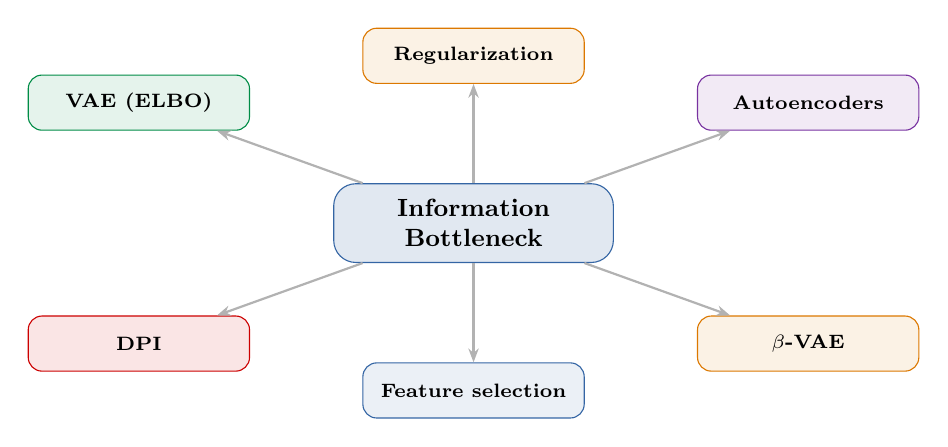
\begin{tikzpicture}[scale=0.85,
  concept/.style={draw=#1, fill=#1!10, rounded corners=5pt, minimum height=0.7cm, text width=2.6cm, align=center, font=\scriptsize\bfseries, inner sep=3pt},
  arr/.style={-{Stealth[length=5pt]}, thick, gray!60},
]
  % Center
  \node[draw=popblue, fill=popblue!15, rounded corners=8pt, minimum height=1cm, text width=3.2cm, align=center, font=\small\bfseries, inner sep=5pt] (ib) at (0, 0) {Information\\Bottleneck};

  % Surrounding concepts
  \node[concept=paramgreen] (vae) at (-5, 1.8) {VAE (ELBO)};
  \node[concept=orange1] (reg) at (0, 2.5) {Regularization};
  \node[concept=violet1] (ae) at (5, 1.8) {Autoencoders};
  \node[concept=sampred] (dpi) at (-5, -1.8) {DPI};
  \node[concept=popblue] (ft) at (0, -2.5) {Feature selection};
  \node[concept=orange1] (bvae) at (5, -1.8) {$\beta$-VAE};

  \draw[arr] (ib) -- (vae);
  \draw[arr] (ib) -- (reg);
  \draw[arr] (ib) -- (ae);
  \draw[arr] (ib) -- (dpi);
  \draw[arr] (ib) -- (ft);
  \draw[arr] (ib) -- (bvae);
\end{tikzpicture}
\end{center}

\vspace{0.1cm}
\begin{center}
\small IB is a \textbf{unifying lens}: many ML techniques can be seen as approximate
solutions to the information bottleneck tradeoff.
\end{center}
\end{frame}

% ============================================================
\section{Summary}

\begin{frame}
\frametitle{Today's Toolbox}

\vspace{-0.15cm}
\begin{center}
\footnotesize
\renewcommand{\arraystretch}{1.5}
\begin{tabular}{lll}
  \textbf{Concept} & \textbf{Key Idea} & \textbf{ML Application} \\
  \hline
  DPI & $X{\to}Y{\to}Z \;\Rightarrow\; I(X;Z) \leq I(X;Y)$ & Layers lose info, sufficient statistics \\
  $f$-divergence & $D_f(p\|q) = \sum q\,f(p/q)$ & Unifies KL, TV, $\chi^2$, Hellinger \\
  Jensen--Shannon & $\text{JSD} = \frac{1}{2}D_{\text{KL}}(p\|m) + \frac{1}{2}D_{\text{KL}}(q\|m)$ & Original GAN objective \\
  ELBO & $\log p(\mathbf{x}) = \text{ELBO} + D_{\text{KL}}(q\|p)$ & VAEs, variational inference \\
  VAE loss & Reconstruction $- \beta\cdot D_{\text{KL}}(q\|p(\mathbf{z}))$ & Generative modeling \\
  Info Bottleneck & $\min I(X;T) - \beta\,I(T;Y)$ & Representation learning \\
  \hline
\end{tabular}
\end{center}

\vspace{0.15cm}
\begin{center}
\fcolorbox{paramgreen}{paramgreen!5}{\parbox{11cm}{\centering\small
  \textbf{The common thread:} Information theory gives us the language to reason about\\
  what neural networks learn, what they forget, and how to train them.\\[3pt]
  DPI says info is lost; IB says lose the right info; ELBO says how to do it in practice.
}}
\end{center}
\end{frame}

% ============================================================
\begin{frame}
\frametitle{Homework}

\begin{enumerate}\setlength{\itemsep}{3pt}
  \item \textbf{DPI application.} Suppose $X \to Y \to Z$ with $I(X;Y) = 2$ bits.
    \begin{itemize}\setlength{\itemsep}{0pt}
      \item[(a)] What is the maximum possible value of $I(X;Z)$?
      \item[(b)] Give an example where $I(X;Z) = I(X;Y)$ (hint: sufficient statistic).
      \item[(c)] Give an example where $I(X;Z) = 0$.
    \end{itemize}

  \item \textbf{$f$-divergences.} Show that the total variation distance
    $\text{TV}(p,q) = \frac{1}{2}\sum|p(x) - q(x)|$ is an $f$-divergence
    with $f(t) = \frac{1}{2}|t - 1|$. Verify $f$ is convex and $f(1) = 0$.

  \item \textbf{ELBO derivation.} Starting from $\log p_\theta(\mathbf{x})$, derive the ELBO
    by writing $\log p_\theta(\mathbf{x}) = \log p_\theta(\mathbf{x}) \cdot \int q_\phi(\mathbf{z}|\mathbf{x})\,d\mathbf{z}$
    and applying Jensen's inequality. Show that the gap is $D_{\text{KL}}(q_\phi \| p_\theta(\mathbf{z}|\mathbf{x}))$.

  \item \textbf{IB tradeoff.} A 10-class classifier uses 128-dim features from a bottleneck layer.
    \begin{itemize}\setlength{\itemsep}{0pt}
      \item[(a)] What is the maximum $I(T;Y)$? (Hint: $H(Y) \leq \log_2 10$.)
      \item[(b)] If we reduce to 2-dim features, how does the IB tradeoff change?
    \end{itemize}
\end{enumerate}
\end{frame}

% ============================================================
\begin{frame}
\begin{center}
  {\Huge\bfseries\textcolor{popblue}{Questions?}}
\end{center}
\end{frame}

\end{document}
